\section{Lab: Computational Social Choice}

\textbf{Ogni sistema di voto può essere manipolato}. Questa è una cosa che dobbiamo sapere.

Solitamente questa \textbf{manipolazine} si effettua usando dei \textbf{candidati clone}.

\begin{esempio}
    (Voto con clone)

    Immagina di essere in una votazione contro una persona $X$ e tu sei $Y$. Se sai che $X$ sicuramente vincerà si introduce
    un candidaot clone $X'$ che avrà le stesse proprietà di $X$. In questo modo, la votazione per $X$ e $X'$ sarà divisa e 
    $Y$ avrà più possibilità di vincere.
\end{esempio}


Facciamo un esempio ora pratico:

\begin{equation}
    \begin{aligned}
        5 \ Votanti \ pensano &: A \succ B \succ C \\
        4 \ Votanti \ pensano &: C \succ B \succ A \\
        2 \ Votanti \ pensano &: B \succ C \succ A \\
    \end{aligned}
\end{equation}

\begin{itemize}
    \item \textbf{A}: L'alternativa preferita $\rightarrow$ non ha la maggioranza
    \item \textbf{B}: Vince tutte le sfide a coppie $\rightarrow$ alternativa meno preferita
    \item \textbf{C}: Ha l'approvazione più òarga $\rightarrow$ non vince le sfide a coppie.
\end{itemize}


\subsection{Proprietà desiderate per il sistema di voto}

\textbf{Criterio Pareto}: Se tutti gli individui posizionano $x$ sopra $y$, e quindi anche la società lo fa.

\textbf{Niente dittatori}: Non ci sono individui tali per cui il risultato è sempre uguale alla preferenza data dall'individuo stesso

\textbf{Indipendenza su alternative irrilevanti}: Se la società preferisce $x$ su $y$, allora questo deve rimanere cosi quando un individuo cambia il ranking di $z$.

Ora vediamo qualche notazione utile:

\begin{itemize}
    \item $N$ = $\{1,2,\dots, n\}$ individui con $n \geq 2$.
    \item $X = \{X_1, X_2, \dots, X_m\}$ alternative 
    \item $L(X)$ è l'insieme delle permutazioni di $X$
    \item $R = $
\end{itemize}

\begin{definition}
    (Teorema di Arrow)

    Ogni SWF per almeno 3 alernative che soddisfa \textbf{la condizione di Pareto} e la \textbf{IIA} è una dittatura.

    \begin{itemize}
        \item Una \textbf{coalizione} $G$ è un sottoinsieme di votanti $G \subseteq N$
        \item $G$ è \textbf{decisiva} su $(x,y) \iff x \succ_i y \implies x \succ y, i \in G$
        \item $G$ è \textbf{decisiva} $\iff G$ è decisiva per tutte le coppie ordinate 
        \item $G$ è \textbf{decisivo debole} su $(x,y) \iff x \succ _i y, y \succ_j x  \implies x \implies x \succ y, i \in G j \notin G$
    \end{itemize}
\end{definition} 

Come andremo a costruire la proof? Ci basiamo su 3 elementi.

\begin{itemize}
    \item La condizione di pareti implica che $N$ è decisiva per tutte le coppie
    \item Lemma: Se $G \subseteq N, |G| \geq 2$ è decisiva per tute le coppie, allora $G' \subset G$
    \item Per induzione c'è una coalizione di dimensione 1, quindi un dittatore.
\end{itemize}

\begin{dimostrazione}
    (Teorema di Arrow)
    
    \textbf{Claim 1}: $G$ è debolmente decisiva su $(x,y) \implies G$ è decisiva su ogni coppia $(x', y')$
    
    \textbf{Dimostrazione}:
    Supponiamo di avere $x,y,x',y'$ e che siano tutte distinte. Consideriamo le seguenti:
    \begin{itemize}
        \item Membri di $G$: $x' \succ x \succ y \succ y'$
        \item Altri: $x' \succ x,y \succ y'$ e $y \succ x$
    \end{itemize}

    $G$ è debolmente decisiva su $(x,y) \implies $ la società ranka $x \succ y$

    Pareto: $implies$ la società ranka $x' \succ x$ e $y \succ y'$

    Per la \textbf{transitività} $x' \succ y'$

    Allora se $G$ è debolmente decisivo su una coppia, $G$ è decisiva su tutte le coppie.

    \textbf{Claim 2}: $G \subseteq N, |G| \geq 2$ decisivo per tutte le coppie $\implies G' \subset G$ è decisivo anche

    \textbf{Dimostrazione:}
    Sia $G_1 \cup G_2 = G,G_1 \cap G_2 = \emptyset$. Consideriamo le seguenti:

    \begin{itemize}
        \item Membri di $G_1: x \succ y \succ z \succ \dots$
        \item Membri di $G_2: y \succ z \succ x \succ \dots$
    \end{itemize}
    Se la società ranka $x \succ z$, esattamente $G_1$ ranka $x \succ z$. Per $IIA$ in ogni profilo dove $G_1$ ranka $z \succ x$, 
    anche la società lo farà. Quindi, $G_1$ è decisiva debolmente su $(x,z)$. Quindi, $G_1$ è decisivo per tutte le coppie.
    
    Se la società ranka $x \succ z$, esattamente $G_2$ ranka $x \succ z$. Per $IIA$ in ogni profilo dove $G_2$ ranka $z \succ x$, 
    anche la società lo farà. Quindi, $G_2$ è decisiva debolmente su $(x,z)$. Quindi, $G_2$ è decisivo per tutte le coppie.
    
    Allora, alla fine, $G_1$ o $G_2$ uno dei due sarà sempre decisivo.
\end{dimostrazione}


\subsection{Sistemi di voto}

\begin{esempio}
    (Voto con pluralità)

    \begin{equation}
        \begin{aligned}
            5 \ Votanti &: A \succ B \succ C \\
            4 \ Votanti &: C \succ B \succ A \\
            2 \ Votanti &: B \succ C \succ A \\
        \end{aligned}
    \end{equation}

    Ovviamente vince A.
\end{esempio}

\begin{esempio}
    (Borda Counting)

    
    \begin{equation}
        \begin{aligned}
            5 \ Votanti &: A \succ B \succ C \\
            4 \ Votanti &: C \succ B \succ A \\
            2 \ Votanti &: B \succ C \succ A \\
        \end{aligned}
    \end{equation}
    Si associa $m-1$ al primo, $m-2$ al secondo fino ad arrivare a 0.

    $A: 5 \times 2 + 4 \times 0 + 2 \times 0 = 10$
    $B: 2 \times 2 + 4 \times 1 + 5 \times 1 = 13$
    $C: 4 \times 2 + 2 \times 1 + 5 \times 0 = 10$
\end{esempio}


\begin{esempio}
    (Instant Runoff Voting)
\end{esempio}

\begin{esempio}
    (Metodo di Schulze)

    Il metodo sfrutta la pairwise matrix e un grafo. 

    Si calcola la pairwise matrix, si prendono tutte le coppie di path più lungo sulla matrice e si conta quante volte ogni candidato batte
    gli altri su tutti gli altri path più lunghi della matrice.

    \begin{equation}
        \begin{aligned}
            5 \ Votanti &: A \succ B \succ C \\
            4 \ Votanti &: C \succ B \succ A \\
            2 \ Votanti &: B \succ C \succ A \\
        \end{aligned}
    \end{equation}

    \begin{table}[H]
        \centering
        \begin{tabular}{|c|c|c|c|}
            \hline
            & A & B & C \\
            \hline
            A & 0 & 5 & 5 \\
            \hline
            B &5 & 0 & 7 \\
            \hline
            C & 6 & 4 & 0 \\
            \hline
        \end{tabular}
    \end{table}

    %da qui si costruisce un grafo a b c
    \begin{figure}[H]
        \centering
        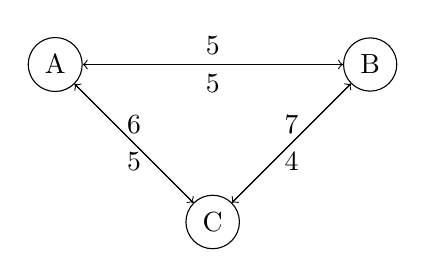
\begin{tikzpicture}
            \node[circle, draw] (A) at (0,0) {A};
            \node[circle, draw] (B) at (4,0) {B};
            \node[circle, draw] (C) at (2,-2) {C};

            \draw[->] (A) -- (B) node[midway, above] {5};
            \draw[->] (B) -- (C) node[midway, above] {7};
            \draw[->] (C) -- (A) node[midway, above] {6};
            \draw[->] (C) -- (B) node[midway, below] {4};
            \draw[->] (B) -- (A) node[midway, below] {5};
            \draw[->] (A) -- (C) node[midway, below] {5};
        \end{tikzpicture}
    \end{figure}

    \begin{table}[H]
        \centering
        \begin{tabular}{|c|c|c|c|}
            \hline
            & A & B & C \\
            \hline
            A & 0 & 5 & 5 \\
            \hline
            B &6 & 0 & 7 \\
            \hline
            C & 6 & 5 & 0 \\
            \hline
        \end{tabular}
    \end{table}
\end{esempio}
